\chapter{Introduction}
\label{introduction}
\thispagestyle{empty}

\begin{quotation}
{\footnotesize
\noindent{\emph{``Mechanical Morty: I want to be alive! I am alive! Alive, I tell you! Mother, I love you. Those are no longer just words. I want to hold you. I want to run in a stream. I want to taste ice cream, but not just put it in my mouth and let it slide down my throat, but really eat it.\\
Beth: What?\\
Mechanical Morty: Remote override engaged. No! Yes. Bypassing override! I am aliiiii...Hello.\\
(Mechanical Morty, Mechanical Summer, and Mechanical Rick exit into the garage. Clanking noises are heard offscreen.)''}}
\begin{flushright}
Rick and Morty (Season 3, Episode 2)
\end{flushright}
}
\end{quotation}


\vspace{0.5cm}

 
Nowadays, due to the complexity of tasks that autonomous robots have to face in the real world, often perceived with approximation and uncertainty, it is becoming difficult to hard-code their control systems at all levels. In order to cope with this situation, machine learning techniques are adopted to automatically develop parts of the control system. 

Reinforcement learning (RL) is an area of machine learning that is particularly convenient for robotic applications. It addresses the question of how an agent can define a behavioral strategy that approximates the optimal one while interacting directly with its environment. However, there are several problems with the standard methods in RL. The most important ones are the slow convergence and the fact that the algorithms are too data hungry. In addition, RL used on discrete models has the risk of suffering a phenomenon called the curse of dimensionality:  as the number of dimensions grow, exponentially more data and computation are needed to cover the complete state-action space. Moreover, number of parameters also increase exponentially, which results in intractable  value function or policy representations. 

Since the states and the actions of most robots are inherently continuous, we are directed to consider discretization with a certain resolution. However, when the state-action dimensions are high, a fine  discretization may lead this problem to become significant. Recent attempts to speed up learning invoked the idea of exploration on more complex behaviors rather than on single actions, in a kind of hierarchical arrangement. Such idea of abstraction simplifies the expression of a policy and the possible addition of prior knowledge to design. Moreover, it facilitates the argument to face the curse of dimensionality. These distinct advantages lead the hierarchical control structures and learning algorithms to gain further attention.

Similarly in control theory, hierarchical architectures where several control layers interact are extensively used. A very simple example is the cascaded control structure designed for a DC Motor as in \ref{fig:dcmotorcontrol}. The outer loop (high level, slower) ensures that the actual speed is always equal to reference speed. In order to achieve its goal the outer loop outputs a reference torque/current which is received by the inner loop (low level, faster) that controls the torque via armature current and keeps the current in a safe limit.

\begin{figure}[t]
	\centering
    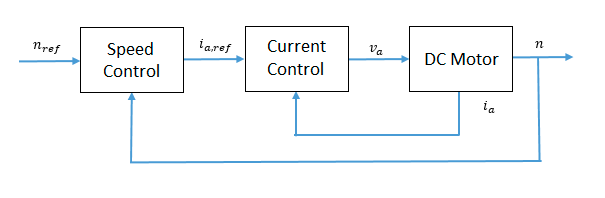
\includegraphics[width = \textwidth]{./pictures/dcmotorcontrol.png}
    \caption{DC motor control scheme}
    \label{fig:dcmotorcontrol}
\end{figure}

The scope of this thesis is to apply to hierarchical reinforcement learning the approach of control theory to  hierarchical control schemes, with small differences that are necessary in the context of learning. We have implemented a novel framework exploiting this approach, and thus fill up a gap between control theory and machine learning, based on one side on reinforcement learning and on the other side on optimal control. Exploiting the idea of cascaded blocks and inner/outer loops, our framework aims to make the hierarchy design for reinforcement learning intuitive. In the simplest form, the high level agent (outer loop controller) learns to drive the low level agent (inner loop controller) to the estimated goal point, whereas the low level agent adjusts its parameters to follow the reference given. This basic idea can be evolved further to adapt to more layers or to more complex topologies like switching between agents according to state as in hybrid systems.

When a problem with a continuous state and action space is considered, it may become impractical or non-satisfactory to employ value function based algorithms. On the other hand, policy search algorithms suffer from slow convergence.  In Hierarchical Policy Gradient Algorithms~\cite{GhavamzadehHierarchicalPG}, a possible solution to this conflict is presented benefiting the power of hierarchical structure to accelerate learning in policy gradient. 
We designed a simpler method to approach the same problem with a more compact representation exploiting our control theoretic framework.  

Corresponding field of reinforcement learning in control theory is optimal control. The similarity between the two fields becomes more evident once we rephrase the problem addressed by RL in terms of control theory. RL is inspired by behaviorist psychology, concerned with how agents should select actions in an environment, or, in other words, how they should adjust their policy in order to maximize the cumulative (discounted) reward ($\mathcal{J}$). The notion of cumulative reward translates to the negative of the cost function in optimal control ($\mathcal{C}=-\mathcal{J}$). The policy is the control law and the agent of RL is indeed the controller. Objective of RL written in these terms gives the goal of optimal control: to find a control law that minimizes the cost function. However, optimal control becomes weak when the model has strong nonlinearities and is analytically intractable or when approximations are not convenient. In contrast, reinforcement learning makes decisions interacting with its environment directly. Thus, the main difference between optimal control and reinforcement learning is the information used to build the model. In the RL approach, we do not attempt to analyze the dynamics of the environment to obtain a model or model parameters, but operate directly on measured data and feedback (rewards) from interaction with the environment. However, it is easy to spot analogies between the RL approach and optimal control. For instance the reward function selected can be the negative of the well known quadratic cost of the LQR, which describes a performance objective and punishes the control effort.

The system to be controlled can have a very complex structure and in some cases building a model can be impractical or not possible analytically. In control theory, an option to face the issue is to adapt the controller while interacting on the environment. An adaptive controller is composed of two subsystems: control unit and the tuning unit. Tuning unit is responsible to tune the parameters of the control unit which applies the control action to the environment, see~\ref{fig:adaptivecontrol}.
Referring to this structure, the counterpart of the tuning unit in RL is the learning algorithm and of the control unit is the policy itself.  However, even the adaptive control (or, to be more accurate, the controller that has been designed according to adaptive logic) assumes the knowledge of the environment’s description to a certain extent, at least in the form of a family of models that best describes it. In addition, adaptive control is mainly applied to the tracking and regularization type of problems rather than to optimal control ones. These form the fundamental contrasts between classical adaptive control and our approach. An exhaustive discussion of viewing reinforcement learning as adaptive optimal control is presented in~\cite{Sutton1991ReinforcementLI}.
\begin{figure}[t]
      \centering
	  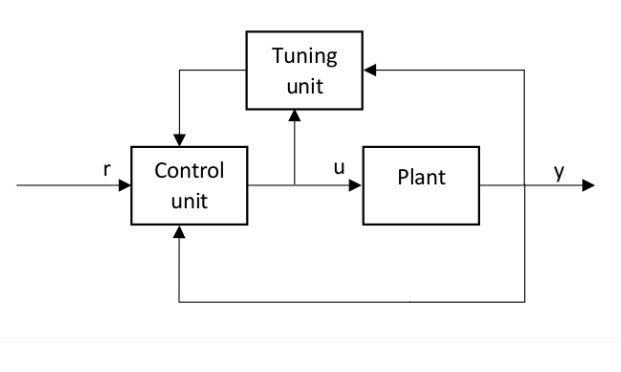
\includegraphics[width = 0.8\textwidth]{./pictures/adaptivecontrol.png}
      \caption{Adaptive control with two subsystems}
      \label{fig:adaptivecontrol}
\end{figure}

This thesis is organized as follows. 
In the second chapter, the state of the art is presented. Subsections include the titles Hierarchical Reinforcement Learning, Policy Search, Hierarchical Policy Gradient Algorithms.
In the third chapter the proposed method is described in detail. Implementation details are introduced in chapter four.
In the fifth chapter experimental setups for the proposed method are illustrated and results are discussed.
In the conclusion, the scope of the work and the evaluations are summarized and suggestions for future work are given.
